%%%%%%%%%%%%%%%%%%%%%%%%%%%%%%%%%%%%%%%%%%%%%%%%%%%%%%%%%%%%%%%%%%%%%%
%
% Institut für Rechnergestuetzte Automation
% Forschungsgruppe Industrial Software
% Arbeitsgruppe ESSE
% http://security.inso.tuwien.ac.at/
% lva.security@inso.tuwien.ac.at
% 
%%%%%%%%%%%%%%%%%%%%%%%%%%%%%%%%%%%%%%%%%%%%%%%%%%%%%%%%%%%%%%%%%%%%%%

\documentclass[12pt,a4paper,titlepage,oneside]{scrartcl}
\usepackage{esseProtocol}

%%%%%%%%%%%%%%%%%%%%%%%%%%%%%%%%%%%%%%%%%%%%%%%%%%%%%%%%%%%%%%%%%%%%%%
%
% FOR STUDENTS
%
%%%%%%%%%%%%%%%%%%%%%%%%%%%%%%%%%%%%%%%%%%%%%%%%%%%%%%%%%%%%%%%%%%%%%%

% Group number or "0" for Lab0
\newcommand{\gruppe}{48}
% Date
\newcommand{\datum}{10.5.2013}
% valid values: "Lab0", "Lab1" (be sure to use Uppercase for first character)
\newcommand{\lab}{Lab1}

% name of course, for example: "IT Security in Large IT Infrastructures", "Security for Systems Engineering", "Introduction to Security"
\newcommand{\lvaname}{Security for Systems Engineering}
% number of course, for example: "183.633", "183.637", "183.594"
\newcommand{\lvanr}{183.637}
% year and term, for example: "SS 2012", "WS 2012", "SS 2013", etc.
\newcommand{\semester}{SS 2013}

% Student data in Lab0 or first student of group in Lab1
\newcommand{\studentAName}{Patrick Fleck}
\newcommand{\studentAMatrnr}{1025484}
\newcommand{\studentAEmail}{e1025484@student.tuwien.ac.at}

% second student of group in Lab1, for Lab0 you may leave it unchanged
\newcommand{\studentBName}{Klaus Behrens}
\newcommand{\studentBMatrnr}{0927376}
\newcommand{\studentBEmail}{e0927376@student.tuwien.ac.at}

% second student of group in Lab1, for Lab0 you may leave it unchanged
\newcommand{\studentCName}{Matthias Pernerstorfer}
\newcommand{\studentCMatrnr}{0929329}
\newcommand{\studentCEmail}{e0929329@student.tuwien.ac.at}

% second student of group in Lab1, for Lab0 you may leave it unchanged
\newcommand{\studentDName}{Martin Winklmüller}
\newcommand{\studentDMatrnr}{1025742}
\newcommand{\studentDEmail}{e1025742@student.tuwien.ac.at}

% second student of group in Lab1, for Lab0 you may leave it unchanged
\newcommand{\studentEName}{David Mihola}
\newcommand{\studentEMatrnr}{9902433}
\newcommand{\studentEEmail}{e9902433@student.tuwien.ac.at}

%%%%%%%%%%%%%%%%%%%%%%%%%%%%%%%%%%%%%%%%%%%%%%%%%%%%%%%%%%%%%%%%%%%%%%
%
% DO NOT CHANGE THE FOLLOWING PART
%
%%%%%%%%%%%%%%%%%%%%%%%%%%%%%%%%%%%%%%%%%%%%%%%%%%%%%%%%%%%%%%%%%%%%%%

\newcommand{\dokumenttyp}{Abgabedokument \lab}

\begin{document}

\maketitle
\setcounter{section}{0}
\setcounter{tocdepth}{2}
\tableofcontents

%%%%%%%%%%%%%%%%%%%%%%%%%%%%%%%%%%%%%%%%%%%%%%%%%%%%%%%%%%%%%%%%%%%%%%
%
% CONTENT OF DOCUMENT STARTS HERE
%
%%%%%%%%%%%%%%%%%%%%%%%%%%%%%%%%%%%%%%%%%%%%%%%%%%%%%%%%%%%%%%%%%%%%%%

\section{Lab1a}

\subsection{Zugang zu Tomcat}
Den Zugang zum Tomcat-Server erhält man sehr leicht - zumindest unter Linux. Alle Arbeiten wurden unter Linux
durchgeführt. Für den Zugang ist es notwendig, sich via SSH auf den ESSE-Server zu verbinden, allerdings mit Port Forwarding
auf den angegebenen Tomcat-Server:

ssh -p 12345 MATRNR@sela.inso.tuwien.ac.at -L 8000:192.168.20.100:8000

Dies hat zur Folge, dass der Port 8000 nun auf den Port des Tomcat-Servers geforwarded wird und es somit ein leichtes
ist, mittels http://localhost:8000 die Homepage auf dem Server einzusehen.

\subsection{Walter's Private Key}
Nun war es die Aufgabe, sich einen SSH-Zugang mit dem User 'walter' zu verschaffen. Hierfür gibt es 2 Möglichkeiten, sich
via SSH zu authentifizieren:
\begin{enumerate}
\item Plain-Text Passwort
\item Private-Key und Public-Key Methode
\end{enumerate}

Natürlich ist es sehr unwahrscheinlich, dass jemand sein Passwort als Plain-Text irgendwo auf einem Server abspeichert. Deshalb
fokussieren wir uns im folgenden auf die 2. Möglichkeit.

Unter Linux-Systemen gibt es hierfür einen Ordner .ssh im Home-Verzeichnis des Users. Im Falle von David Mihola würde
dieser unter /home/David/.ssh zu finden sein. Hier liegt nun eine Datei id\_rsa, die im Normalfall den Private Key
des Users, der den SSH-Zugang anfordert beinhaltet.

Nun sollte es doch für 'walter' genauso sein. Das heißt wir suchen nach dem Ordner /home/walter/.ssh. Dieser ist aber
natürlich am Server geschützt und kann nicht einfach durch eintippen in Plain-Text in die Adresse des Servers
angesurft werden. Jedoch hat der hier verwendete Tomcat-Server eine Schwachstelle. Mittels Directory-Traversal kann
der Server ausgetrickst werden und der Ordner eingesehen werden. Hier die Adresse der zu untersuchenden Datei:
\url{http://localhost:2222/%c0%ae%c0%ae/%c0%ae%c0%ae/%c0%ae%c0%ae/%c0%ae%c0%ae/%c0%ae%c0%ae/home/walter/.ssh/id\_rsa}

Directory-Traversal führt hier eine Umwandlung von Plain-Characters in Sonderzeichen ein, wodurch der Server nun die Datei auch
anzeigt. Die Sonderzeichen sind spezielle URI-Zeichenfolgen, die vom Server in Plain-Text umgewandelt werden. Damit kann
man etwaige Schutzmechanismen des Tomcat-Servers umgehen.

\subsection{SSH-Zugang via User 'Walter'}
Wie bekommt man nun einen SSH-Zugang mit einem fremden Private Key?
Wie oben beschrieben, gibt es für jeden User den Ordner .ssh mit den Private Keys für SSH-Zugängen. Es muss nun
möglich sein, sich einen Zugang zum User 'walter' zu verschaffen, indem man sich als dieser ausgibt. Dazu
wird einfach im Ordner /home/David/.ssh eine Datei namens id\_rsa erstellt (falls diese noch nicht existiert). Danach wird
der gefundene Schlüssel von 'walter' hineinkopiert und die Datei gespeichert. Nun ist es noch notwendig mittels 'chmod
600 id\_rsa' den Zugriffsschutz des Keys auf Permission 600 umzustellen. Andernfalls wird der Server die Verbindung
verweigern, da der Key nicht ausreichend geschützt ist. Das Port-Forwarding über die SSH-Verbindung zum ESSE-Institut
sollte nun noch vorhanden sein. Da wir ja über den Port 2222 direkt auf den Tomcat-Server zugreifen können, ist es nun
möglich, sich mittels 'ssh -p 2222 walter@localhost' mit dem Benutzer 'walter' einzuloggen. Dies funktioniert aus folgendem
Grund:\linebreak
Auf dem Server befinden sich (in der Datei \url{~/.ssh/authorized_keys}) die Public-Key aller User, die mittels Public-Key/Private-Key Zugang zum Server bekommen sollen. Wird nun eine Verbindung angefordert, so muss der User, der dies durchführt, einen Private-Key in seinem .ssh-Ordner besitzen, der zu einem Public-Key am Server passt.
Wir haben uns den Private-Key von 'walter' in unseren eigenen .ssh-Ordner kopiert und der Server glaubt nun, wir seien
auch dieser User.

\subsection{Analyse}
In diesem Abschnitt wird besprochen, welche Fehler zu den genannten Sicherheitslücken geführt haben, und wie sie behoben werden können. Es handelt sich um drei mehr oder weniger unabhängige Fehler, wobei schon das Beheben eines einzigen dieser Fehler das Eindringen erheblich erschweren würde.

\subsubsection{Fehler1: Veraltete Tomcat-Version}
Die verwendete Version des Tomcat-Servers (6.0.16) hat offentsichtlich eine Sicherheitslücke, die den Zugriff auf Dateien erlaubt, die außerhalb der Ordners für Web-Dokumente auf dem Server liegen. Ein Update auf eine aktuelle(re) Version des Servers hätte diese Lücke geschlossen und damit verhindert, dass über den Webserver auf beliebige User-Daten - wie z. B. Walters privaten SSH-Schlüssel - zugegriffen werden kann.

\subsubsection{Fehler 2: Privater SSH-Key auf dem Server}
Die Bezeichnung "privater Schlüssel" hätte für Walter ein ausreichender Hinweis sein müssen, um diesen privaten Schlüssel an einem \emph{privaten} Ort abzulegen. Ein über das Internet zugänglicher Server ist nicht so ein privater Ort. Darüberhinaus ist es nicht nur gefährlich, sondern auch sinnlos, den privaten Schlüssel auf jenem Rechner aufzubewahren, für den er den Zugang ermöglicht.
Walter hätte also nur eine Kopie seines öffentlichen Schlüssels (in der Datei \url{~/.ssh/authorized_keys}) auf dem Server belassen sollen. Den privaten Schlüssel hätte er vom Server löschen müssen und ihn \emph{nur auf dem Rechner, von dem aus er Zugriff auf den Server haben möchte}, aufbewahren sollen.

\subsubsection{Fehler 3: Privater SSH-Key nicht passwortgeschützt}
Die vorherigen beiden Sicherheitslücken wären noch längst nicht so gravierend ausgefallen, hätte Walter seinen Schlüssel wenigestens durch ein ausreichend starkes Passwort geschützt. Stattdessen verwendete der Schlüssel die sogenannte "empty passphrase", also gar kein Passwort, wie ein kurzer Angriff mit dem Tool phrasendrescher verriet:

\begin{lstlisting}
david@brazos:~/lab1$ phrasendrescher -i 8 id_rsa
phrasen|drescher 1.0 - the passphrase cracker
Copyright (C) 2007 Nico Leidecker; nfl@portcullis-security.com

match: (0) id_rsa {empty passphrase}
finished!
bye, bye...
\end{lstlisting}

Walter hätte also ein ausreichend starkes Passwort - oder eben besser gleich eine längere Passphrase - wählen sollen, um seinen Schlüssel zu schützen. Dann hätte selbst ein Angreifer, der beide anderen Sicherheitslücken ausnützen konnte, den Schlüssel nicht verwenden können.

Letztlich war der Angriff also nur durch das Zusammenspiel von 3 einzelnen Sicherheitslücken möglich.



\section{Lab1b - Netzwerkanalyse}

\subsection{Direkt erreichbare Netze}

Im ersten Schritt war zu ermitteln, welche Netzwerke vom Tomcat-Server aus direkt zu erreichen sind. Die Antwort darauf liefert das Auslesen der sogenannten Kernel Routing Tables mit Hilfe von netstat.

\begin{lstlisting}
walter@tomcat:~$ netstat -rn
Kernel IP routing table
Destination     Gateway         Genmask         Flags   MSS Window  irtt Iface
192.168.20.0    0.0.0.0         255.255.255.0   U         0 0          0 eth0
192.168.98.0    0.0.0.0         255.255.255.0   U         0 0          0 eth1.98
0.0.0.0         192.168.98.1    0.0.0.0         UG        0 0          0 eth1.98
walter@tomcat:~$ netstat -6rn
Kernel IPv6 routing table
Destination                    Next Hop                   Flag Met Ref Use If
fdcb:c447:e9d2:3553:1001::/120 ::                         U    256 0
  1 eth1.98
fe80::/64                      ::                         U    256 0     0 eth0
fe80::/64                      ::                         U    256 0     0 eth1
fe80::/64                      ::                         U    256 0
  0 eth1.98
::/0                           fdcb:c447:e9d2:3553:1001::1 UG   1024
1224143 eth1.98
::/0                           ::                         !n   -1  1246254 lo
::1/128                        ::                         Un   0   3    28 lo
fdcb:c447:e9d2:3553:1001::ab/128 ::                         Un   0   1 76668 lo
fe80::21b:d7ff:fe12:bc52/128   ::                         Un   0   1  2235 lo
ff00::/8                       ::                         U    256 0     0 eth0
ff00::/8                       ::                         U    256 0     0 eth1
ff00::/8                       ::                         U    256 0
  0 eth1.98
::/0                           ::                         !n   -1  1246254 lo
\end{lstlisting}

Die direkt erreichbaren Netze sind daher: 192.168.20.0/24, 192.168.98.0/24 und 

\subsection{Ping-Scan}

Im nächsten Schritt war ein Ping-Scans durchzuführen, um zu ermitteln, welche Hosts in den genannten IP-Adress-Bereichen erreichbar sind. Die zu durchsuchenden Bereich waren dabei: 192.168.96.0/21, 172.16.0.0/22, 10.12.0.0/24 für IPv4 sowie fdcb:c447:e9d2:3553:1000::/120 bis fdcb:c447:e9d2:3553:100f::/120.

Die Scans der IPv4-Adresse konnten wir direkt auf dem Server durchführen:

\begin{lstlisting}
walter@tomcat:~$ nmap -v -sP 192.168.96.0/21 | grep up
Host omega.local.vienna.essecorp.invalid (192.168.98.1) is up (0.0023s latency).
Host alpha.local.vienna.essecorp.invalid (192.168.98.10) is up (0.00054s latency).
Host beta.local.vienna.essecorp.invalid (192.168.98.28) is up (0.00023s latency).
Host gamma.local.vienna.essecorp.invalid (192.168.98.54) is up (0.00035s latency).
Host delta.local.vienna.essecorp.invalid (192.168.98.99) is up (0.0031s latency).
Host tomcat.local.vienna.essecorp.invalid (192.168.98.124) is up (0.000076s latency).
Host epsilon.local.vienna.essecorp.invalid (192.168.98.201) is up (0.00038s latency).
Host zeta.local.vienna.essecorp.invalid (192.168.98.202) is up (0.0015s latency).
Nmap done: 2048 IP addresses (8 hosts up) scanned in 87.47 seconds

walter@tomcat:~$ nmap -v -sP 172.16.0.0/22 | grep up
Host gemini.dmz.vienna.essecorp.invalid (172.16.2.12) is up (0.0065s latency).
Host phoenix.dmz.vienna.essecorp.invalid (172.16.2.15) is up (0.0035s latency).
Host taurus.dmz.vienna.essecorp.invalid (172.16.2.25) is up (0.0041s latency).
Host lyra.dmz.vienna.essecorp.invalid (172.16.2.253) is up (0.00070s latency).
Nmap done: 1024 IP addresses (4 hosts up) scanned in 78.61 seconds

walter@tomcat:~$ nmap -v -sP 10.12.0.0/24 | grep up
Nmap done: 256 IP addresses (0 hosts up) scanned in 104.14 seconds
\end{lstlisting}

Da nmap beim Scan von IPv6-Adressen keine Adressebereiche unterstütz, mussten wir uns für diesen Teil der Aufgabe ein kleines Python-Skript schreiben, das die gewünschten Adressen erzeugt und dann für jede einzelne Adresse nmap aufruft.
Eine weitere Komplikation ergab sich, da wir auf dem Tomcat-Server keinerlei Schreibrechte hatten. Aus diesem Grund konnten wir weder das Skript selbst auf dem Server ablegen, noch den Output des Skripts in eine Datei auf dem Server schreiben, um sie später zur Analyse zur Verfügung zu haben. Um dies zu umgehen, ließen wir das Skript auf einem unserer Rechner lokal laufen und riefen im Skript nmap über ssh auf dem Server auf:

\begin{lstlisting}
import subprocess

for y in range (0, 16):
  base_address = "fdcb:c447:e9d2:3553:100" + format(y, 'x') + ":0000:0000:00"
  for x in range (0, 256):
    address = base_address + format(x, 'x')
    subprocess.call(['ssh', '-p 2222', 'walter@localhost', 'nmap', '-6', '-sP', address])
\end{lstlisting}

Der Aufruf des Skripts bringt folgendes Ergebnis:

\begin{lstlisting}
david@brazos:~/lab1$ python ipv6-scan.py > output.txt
david@brazos:~/lab1$ cat output.txt | grep fdcb
Host omega.local.vienna.essecorp.invalid (fdcb:c447:e9d2:3553:1001::1) is up (0.0041s latency).
Host alpha.local.vienna.essecorp.invalid (fdcb:c447:e9d2:3553:1001::5) is up (0.0044s latency).
Host beta.local.vienna.essecorp.invalid (fdcb:c447:e9d2:3553:1001::9) is up (0.0041s latency).
Host gamma.local.vienna.essecorp.invalid (fdcb:c447:e9d2:3553:1001::21) is up (0.0027s latency).
Host delta.local.vienna.essecorp.invalid (fdcb:c447:e9d2:3553:1001::43) is up (0.0064s latency).
Host epsilon.local.vienna.essecorp.invalid (fdcb:c447:e9d2:3553:1001::79) is up (0.0064s latency).
Host zeta.local.vienna.essecorp.invalid (fdcb:c447:e9d2:3553:1001::88) is up (0.0064s latency).
Host tomcat.local.vienna.essecorp.invalid (fdcb:c447:e9d2:3553:1001::ab) is up (0.000044s latency).
Host lyra.dmz.vienna.essecorp.invalid (fdcb:c447:e9d2:3553:1002::fd) is up (0.00021s latency).
Host kerberos.dmz.vienna.essecorp.invalid (fdcb:c447:e9d2:3553:1002::fe) is up (0.00049s latency).
Host athena.extra.atlanta.essecorp.invalid (fdcb:c447:e9d2:3553:1003::7f) is up (0.26s latency).
Host zeus.extra.atlanta.essecorp.invalid (fdcb:c447:e9d2:3553:1003::9a) is up (0.27s latency).
Host kerberos.extra.atlanta.essecorp.invalid (fdcb:c447:e9d2:3553:1003::da) is up (0.00046s latency).
\end{lstlisting}

\subsection{Port-Scans}
Als nächstes scannten wir alle gefundenen Hosts auf offene Ports und laufende Services.
Nachfolgend werden die gefundenen IP-Adressen und ihre zugehörigen offenen Ports sowie Services aufgelistet:
TCP IPv4 Scans:
\begin{lstlisting}
192.168.98.10 Port 53 domain dnsmasq 2.55
192.168.98.28 Port 25 SMTP
192.168.98.54 Port 1080 socks5 (Username/password authentication required)
192.168.98.99 Port 631 ipp cups 1.4 (Printserver Apple)
192.168.98.124 Port 8000 Apache Tomcat/Coyote JSP engine 1.1
192.168.98.124 Port 8009 ajp13 Apache Server, Service Info: OS: Linux 
192.168.98.124 Port 22 OpenSSH 5.5p1 Debian 6+sqeueeze3 (Protocol 2.0), OS: Linux
192.168.98.201 Port 139 und 445 (Printserver smb mit und ohne netbios) netbios-ssn Samba smbd 3.X (workgroup: ESSECORP)
172.16.2.12 http lighttpd 1.4.28 dmz
172.16.2.15 Port 21 FTP vsftpd 2.3.2 dmz
172.16.2.25 Port 25 SMTP dmz
\end{lstlisting}

IPv6 Scans:
\begin{lstlisting}
athena.extra.atlanta.essecorp.invalid:
Port 80 - http ligthttpd
Port 443 - ssl/http lighttpd
lighthttpd ist ein kleiner Webserver, der Perl, PHP, Python und Ruby unterstützt

zeus.extra.atlanta.essecorp.invalid:
Port 7 - echo
Port 9 - discard?
Port 13 - daytime
Port 19 - chargen Linux
Port 22 - ssh
Port 37 - time?
\end{lstlisting}

Der Netzwerkplan zeigt wie das Netzwerk aufgebaut ist.

\begin{figure}[h!]
  \centering
  \fbox{
    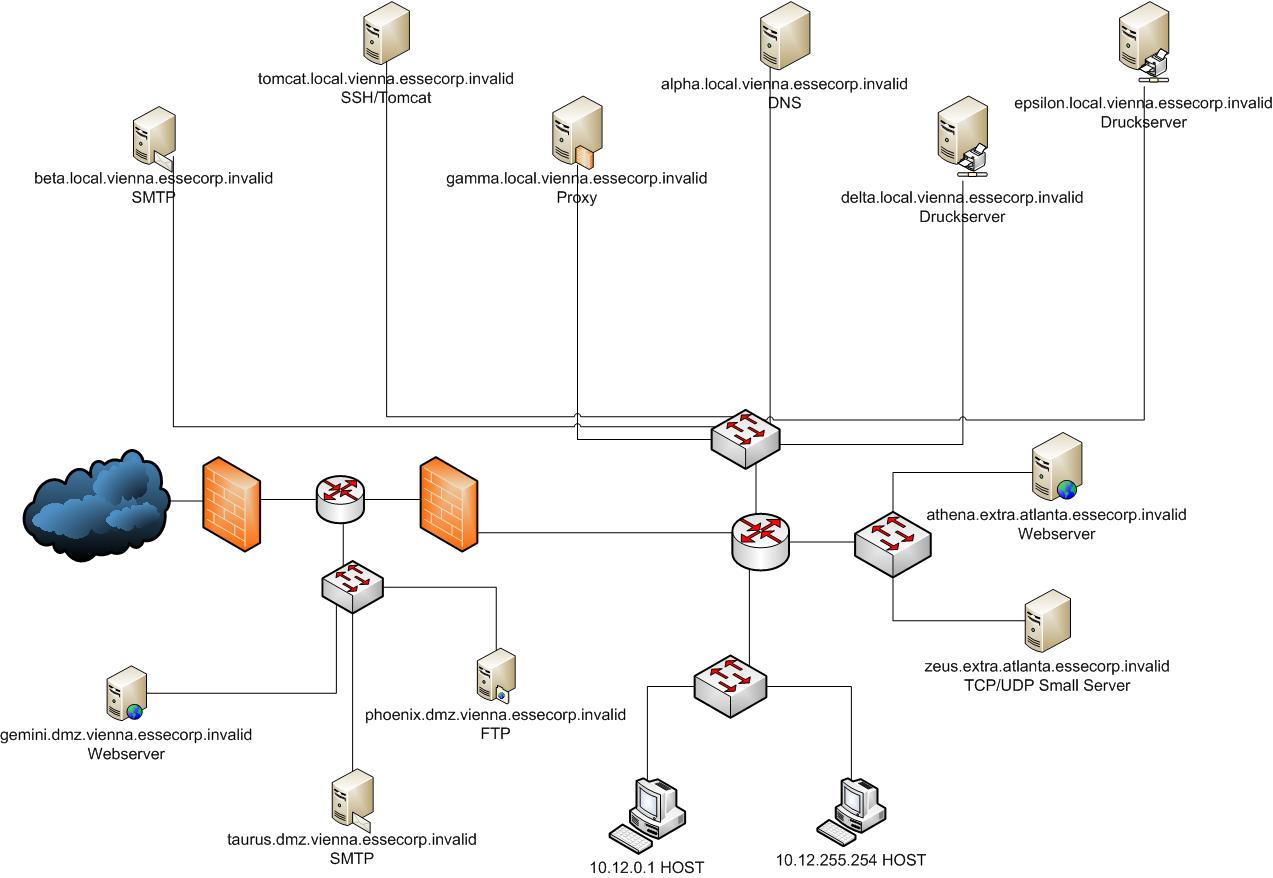
\includegraphics[width=1\textwidth]{./imgs/Netzwerkplan.jpg}
  }
  \caption{Netzwerkplan}
  \label{fig:netzwerkplan}
\end{figure}

Es fällt sofort auf, dass es 4 verschiedene große Domänen gibt, die jeweils eine andere Funktionalität verfolgen:
\begin{enumerate}
\item local.vienna.essegroup.invalid
\item dmz.vienna.essegroup.invalid
\item extra.atlanta.essegroup.invalid
\item Hosts
\end{enumerate}

Die erste lokale Domäne beinhaltet einen typischen Proxy, der innerhalb des lokalen Netzwerkes arbeitet. Außerdem gibt es einen
internen Mail-Server (SMTP), einen internen Tomcat mit SSH-Zugang, sowie den typischen DNS und 2 Druckerserver, die
nur intern genutzt werden können.\linebreak
Die DMZ (Demilitarisierte Zone) bietet Services an, auf die man auch aus dem Internet zugreifen kann. Somit existieren die
3 Komponenten Mailserver, FTP- und SMTP-Server.\linebreak
Die Komponenten TCP/UDP-Server, sowie ein kleiner Lightweight-HTTP-Webserver liegen hier in einer eigenen Domäne.\linebreak
Die Host bekommen Adressen im Bereich von 10.12.0.1 bis 10.12.255.254.


\include{lab1c}

\section{Ueberschrift 2}

\subsection{Sub-Ueberschrift 1}
Lorem ipsum dolor sit amet, consetetur sadipscing elitr, sed diam nonumy eirmod tempor invidunt ut labore et dolore magna aliquyam erat, sed diam voluptua. 

\subsection{Sub-Ueberschrift 2}
Lorem ipsum dolor sit amet, consetetur sadipscing elitr, sed diam nonumy eirmod tempor invidunt ut labore et dolore magna aliquyam erat, sed diam voluptua. At vero eos et accusam et justo duo dolores et ea rebum. 

\subsection{Sub-Ueberschrift 3}
Lorem ipsum dolor sit amet, consetetur sadipscing elitr, sed diam nonumy eirmod tempor invidunt ut labore et dolore magna aliquyam erat, sed diam voluptua. 

\section{Beispiele}

\subsection{Source Code formatieren}
Es folgen einige Beispiele wie Sourcecode in diesem Dokument formatiert und referenziert werden kann
(\hyperref[code:beispiel1]{siehe Listing~\ref*{code:beispiel1} auf Seite~\pageref*{code:beispiel1}} und \hyperref[code:beispiel2]{siehe Listing~\ref*{code:beispiel2} auf Seite~\pageref*{code:beispiel2}}).

Ebenso können kurzer Code oder kurze Befehle direkt in der Zeile in einem \lstinline{lstinline Block} mit typengleicher Schrift formatiert werden.

\lstinputlisting[caption=Example C/C++ file,label=code:beispiel1,style=c]{example.c}

\begin{lstlisting}[caption=Example bash script,label=code:beispiel2,style=simple]
#!/bin/bash
echo "Bash version ${BASH_VERSION}..."
for i in {0..10..2}
  do
     echo "Welcome $i times"
 done

echo "some very very very very very very very very very very very very very very very very very very very very long string"

exit 0;
\end{lstlisting}

\subsection{Bilder}

Es folgen einige Beispiele wie Bilder in diesem Dokument eingefuegt werden koennen
(\hyperref[fig:logo1]{siehe Abbildung~\ref*{fig:logo1} auf Seite~\pageref*{fig:logo1}}).

\begin{figure}[h!]
  \centering
  \fbox{
    
\includegraphics[width=0.4\textwidth]{./imgs/esse-logo-bw.png}
  }
  \caption{ESSE Logo}
  \label{fig:logo1}
\end{figure}


\end{document}


